% 文档类设置
\documentclass{ctexart}

% 导入宏包
\usepackage{hyperref} % PDF标签
\usepackage{graphicx} % 图片
\graphicspath{{images/}} % 图片路径
\usepackage{geometry} % 页面边距宏包
\geometry{left=3.17cm,right=3.17cm,top=2.54cm,bottom=2.54cm} % 页边距
\usepackage{fancyhdr} % 页眉页脚
\pagestyle{fancy} % 页面样式
\cfoot{\thepage} % 页脚中部
\renewcommand\headrulewidth{0pt}%隐藏页眉横线
\usepackage{enumerate} % 编号列表
\usepackage[simplified]{pgf-umlcd} % UML
\usepackage{listings} % 代码排版
\usepackage{dirtree} % 绘制树形目录
\usepackage{url} % 超链接
\usepackage{color,xcolor} % 颜色宏包
\usepackage[ruled]{algorithm2e} % 算法环境
% \usepackage{algorithmic} % 算法描述
% 代码块风格
\lstset{
    numbers=left,           % 行号
    numberstyle=\tiny,      % 行号样式
    basicstyle=\ttfamily,   % 基本代码风格
    breaklines=true,        % 自动换行
    keywordstyle=\bfseries\color{green!40!black}, % 关键字风格
    commentstyle=\itshape\color{gray}, % 注释的风格
    identifierstyle=\bfseries\color{blue}, % 标识符风格
    stringstyle=\color{orange}, % 字符串风格
    columns=fixed,
    frame=single, % 显示边框
    xleftmargin=\parindent,  % 左边距
    % xrightmargin=\parindent, % 右边距
    aboveskip=1em, % 顶部间隔
    captionpos=b % 文字提示符
}
\renewcommand{\lstlistingname}{代码}

% 算法描述的设置
\SetAlgorithmName{算法}{算法}{算法列表}
\SetKwInput{KwIn}{输入}
\SetKwInput{KwOut}{输出}
\LinesNumbered


% 角注设置
% \renewcommand{\thefootnote}{\fnsymbol{footnote}}

% 章节标题设置
\ctexset{
    section = {
        format+ =  \zihao{-3} \raggedright,
        name = {,\quad},
        number = \arabic{section},
        aftername = \hspace{0pt}
    },
    subsection = {
        format+ =  \zihao{4} \raggedright,
        name = {,\quad},
        number = \arabic{section}.\arabic{subsection},
        aftername = \hspace{0pt}
    },
    subsubsection = {
        format+ =  \zihao{-4} \raggedright,
        name = {,\quad},
        number = \arabic{section}.\arabic{subsection}.\arabic{subsubsection},
        aftername = \hspace{0pt}
    }
}

% 封面页
\newcommand{\makecover}[4]{
    \begin{titlepage}
        \centering
        
\includegraphics[width=0.5\textwidth]{logo.png}\par
        \vspace{1cm}
        {\kaishu\ziju{0.1}\Huge 数学与计算机学院}\par
        \vspace{5.0cm}
        {\bfseries\ziju{0.1}\zihao{-0} #1}\par
        \vspace{5.0cm}
        {\kaishu\ziju{0.1}\Huge #2}\par
        \vspace{0.7cm}
        {\kaishu\Large #3}\par
        \vspace{1em}
        {\kaishu\large #4}\par
        \vspace{2em}
        {\itshape 本作品采用 \href{https://creativecommons.org/licenses/by-nc-sa/4.0/}{CC-BY-NC-SA} 协议进行许可}\par
        \vspace{1em}
        
\includegraphics[width=0.2\textwidth]{cc-by-nc-sa.png}
    \end{titlepage}
}

% 画UML类图
% 参数2:文本宽度,参数3:类名,参数1:左上角坐标
\newenvironment{UMLClass}[3][0,0]
{
    \vspace{1em}\par\ttfamily
    \begin{tikzpicture}
        \begin{class}[text width=#2]{#3}{#1}
}
{
        \end{class}
    \end{tikzpicture}
    \vspace{1em}
}


\begin{document}
    % 产生封面
    \makecover{哈夫曼编(译)码系统\par \vspace{0.3em}设计报告}{杨鑫}{计算机11902班}{\today}
    
    \section{需求分析}
    \subsection{问题描述}
    利用哈夫曼编码进行通信可以大大提高信道利用率,缩短信息传输时间,降低传输成本。
    但是,这要求在发送端通过一个编码系统对待传数据预先编码,在接收端将传来的数据进行译码(解码)。
    对于双工信道(即可以双向传输信息的信道),每端都需要一个完整的编/译码系统。
    试为这样的信息收发站设计一个哈夫曼编译码系统。
    
    \subsection{基本要求}
    \begin{enumerate}[\indent (1)]
        \item 初始化(Initialization)
        \par 从数据文件DataFile.data中读入字符及每个字符的权值,建立哈夫曼树HuffTree;
        \item 编码(EnCoding)
        \par 用已建好的哈夫曼树,对文件ToBeTran.data中的文本进行编码形成报文,将报文写在文件Code.txt中;
        \item 译码(DeCoding)
        \par 利用已建好的哈夫曼树,对文件CodeFile.data中的代码进行解码形成原文,结果存入文件Textfile.txt中;
        \item 输出(Output)
        \par 输出DataFile.data中出现的字符以及各字符出现的频度(或概率);
        \par 输出ToBeTran.data及其报文Code.txt;
        \par 输出CodeFile.data及其原文TextFile.txt。
    \end{enumerate}

    \section{概要设计}
    \subsection{数据结构}
    \subsubsection{哈夫曼树结点}
    本系统的关键实现取决于构造一棵哈夫曼树。哈夫曼树的一个结点包括权值,父结点,左右孩子结点。
    假设由$n$个字符来构造一棵哈夫曼树,则共有结点$2n-1$个。我们以线性结构实现哈夫曼树,
    详见下文描述。

    哈夫曼树结点的数据成员:
    \begin{itemize}
        \item ch:当前结点代表的字符,根据哈夫曼树的特点,非叶子结点值为空
        \item weight:当前结点的权值
        \item parent:当前结点的父结点序号,若无父结点,设其为0
        \item lchild:当前结点的左孩子结点序号,若无左孩子,设其为0
        \item rchild:当前结点的右孩子结点序号,若无右孩子,设其为0
    \end{itemize}
    
    \begin{center}
        \begin{UMLClass}{8cm}{HTNode}
            \attribute{+ ch: string}
            \attribute{+ weight: size\_t}
            \attribute{+ parent: size\_t}
            \attribute{+ lchild: size\_t}
            \attribute{+ rchild: size\_t}
        \end{UMLClass}
        \footnote{size\_t是无符号超长整型,即 unsigned long long 。}
    \end{center}

    \subsubsection{系统综合结构}
    实现哈夫曼编(译)码系统,主要依据一棵哈夫曼树,以及其生成的哈夫曼编码表。
    将上述多个数据结构,以及相应的构造、编码、译码算法封装,形成一个“哈夫曼编码树”类。
    这些算法将在下节论述。

    \begin{center}
        \begin{UMLClass}{10cm}{Huffman}
            \attribute{- tree: HTNode*}
            \attribute{- size: size\_t}
            \attribute{- code: string*}
            \operation{- totalSize(): size\_t}
            \operation{- select(n: size\_t, s1: size\_t\&, s2: size\_t\&)}
            \operation{- init(n: size\_t, \_ch: string*, \_weight: size\_t*)}
            \operation{+ Huffman()}
            \operation{+ Huffman(n: size\_t, \_ch: string*, \_weight: size\_t*)}
            \operation{+ Huffman(is: istream\&)}
            \operation{+ operator=(h: Huffman\&\&): Huffman\&}
            \operation{$\sim$ Huffman()}
            \operation{+ printTree()}
            \operation{- enCode()}
            \operation{+ enCode(is: istream\&): string}
            \operation{+ enCode(str: const string\&): string}
            \operation{+ printCode()}
            \operation{+ deCode(is: istream\&): string}
            \operation{+ deCode(str: const string\&): string}
        \end{UMLClass}
    \end{center}

    Huffman 类数据成员:
    \begin{itemize}
        \item tree:一棵以动态数组实现的哈夫曼树,数组下标即代表了当前的序号,0号单元不使用
        \item size:字符数,也代表叶子结点数,假定n个,则对应1$\sim$n单元结点的字符值非空
        \item code:存储各字符编码后的二进制编码,因为tree的0号单元不使用,所以表长为字符数加1
    \end{itemize}

    Huffman 类成员函数:
    \begin{itemize}
        \item totalSize:计算tree的总大小,等同于2*size+1,即tree结点总数
        \item select:将两个双亲域为0且权值最小的结点的下标赋给参数 s1, s2
        \item init:初始化哈夫曼树
        \item Huffman:构造哈夫曼树,可以多种方式构造(从字符和权值数组、从输入流)
        \item operator=:移动复制操作符,将右值引用复制给当前Huffman对象
        \item printTree:输出当前Huffman对象的关键参数(各结点的字符值、权值、父子结点序号)
        \item enCode:编码,可以是对系统所有字符编码,或者,对输入的一串字符串进行编码;
        \par 在构造哈夫曼树时,就经历了初始化(init)和编码(enCode)阶段。
        \item printCode(): 输出系统各字符的二进制编码
        \item deCode:译码,翻译二进制字符串
    \end{itemize}

    \subsection{算法}
    \subsubsection{构造哈夫曼树}
    假如由n个字符来构造一棵哈夫曼树,则共有结点2n-1个。
    
    构造哈夫曼树的操作是,将1$\sim$n号结点作为叶子结点,输入各结点的字符、权值。
    并将他们的parent、lchild、rchild均赋值为0。

    然后,在当前哈夫曼树中选择权值最小且双亲域为0的两个结点作为下一结点的子结点,
    新结点的权值为这两个结点的权值之和。

    将上述操作称哈夫曼树的初始化算法,见算法描述\ref{alg1}。

    然后进行对各字符的编码操作(见下一小节)。

    \subsubsection{编码}
    编码操作一,生成构造哈夫曼树的各个字符\footnote{此处为方便系统实现,用"(space)"(不含引号)表示在编码表中的空格字符。}的编码表。

    编码操作一的思想是“\emph{逆序编码}”,从叶子结点出发,向上回溯,如果该结点是回溯到上一个结点的左孩子,
    则在记录编码的字符串里追加“0”,否则追加“1”,注意是倒着追加;
    直到遇到根结点(结点双亲为0),每一次循环编码到根结点,把编码存在编码表中,
    然后开始编码下一个字符(叶子)。

    详见算法描述\ref{alg2}。

    编码操作二,对输入的一串字符串编码,此时,只需遍历该字符串,在编码表寻找每个字符对应的二进制编码,
    然后将这些二进制编码“串接”在一块。

    \subsubsection{译码}
    译码的思想是循环读入一串哈夫曼序列,读到“0”从根结点的左孩子继续读,
    读到“1”从右孩子继续,如果读到一个结点的左孩子和右孩子是否都为0,
    说明已经读到了一个叶子(字符),翻译一个字符成功,
    把该叶子结点代表的字符追加到一个字符串中,然后继续从根结点开始读,
    直到读完这串哈夫曼序列。如果读到最后哈夫曼序列的最后一个位置,却不是叶子结点,
    说明不是一个有效的哈夫曼序列。详见算法描述\ref{alg3}。
    
    % 初始化
    \begin{algorithm}[p]
        \caption{初始化哈夫曼树}
        \label{alg1}
        \KwIn{字符数 n, 字符数组 ch, 权值数组 weight}
        \eIf{$n<=1$}{
            字符数过少,无法初始化\;
            STOP\;
        }{$size \gets n$}
        为tree分配$2*size - 1$的存储空间\;
        \For{$i \gets 1$ \KwTo 2*size - 1}{
            \If{$i <= size$}{
                $tree[i].ch \gets ch[i-1]$\; 
                $tree[i].weight \gets weight[i-1]$\; 
            }
            $tree[i].lchild \gets 0$\;
            $tree[i].rchild \gets 0$\;
            $tree[i].parent \gets 0$\;
        }
        \For{$i \gets size + 1$ \KwTo 2*size - 1}{
            选择权值最小且双亲域为0的结点s1,s2\;
            $tree[s1].parent \gets i$\;
            $tree[s2].parent \gets i$\;
            $tree[i].lchild \gets s1$\;
            $tree[i].rchild \gets s2$\;
            $tree[i].weight \gets tree[s1].weight + tree[s2].weight$\;
        }
    \end{algorithm}
    % 编码
    \begin{algorithm}[hp]
        \caption{编码}
        \label{alg2}
        \KwOut{编码表}
        为编码表code分配$size + 1$的存储空间\;
        \For{$i \gets 1$ \KwTo size}{
            $current \gets i$\;
            $father \gets tree[current].parent$\;
            \While{$father != 0$}{
                \eIf{$tree[father].lchild == c$}{
                    在code[i]的初始位置插入字符'0'\;
                }{
                    在code[i]的初始位置插入字符'1'\;
                }
                $current \gets father$\;
                $father \gets tree[father].parent$\;
            }
        }
    \end{algorithm}
    % 译码
    \begin{algorithm}[hp]
        \caption{译码}
        \label{alg3}
        \KwIn{二进制哈夫曼序列str}
        \KwOut{翻译后的字符串ans}
        $q \gets totalSize()$\;
        \For{$i \gets 0$ \KwTo str的长度 - 1}{
            \While{$father \neq 0$}{
                \uIf{$str[i] == '0'$}{
                    $q \gets tree[q].lchild$\;
                }
                \uElseIf{$str[i] == '0'$}{
                    $q \gets tree[q].rchild$\;
                }
                \Else{
                    抛出异常\;
                }
            }
            \uIf{tree[q]为叶子结点}{
                $ans += tree[q].ch$\;
                $q \gets totalSize()$\;
            }
            \ElseIf{$i == str.size() - 1$}{
                抛出异常\;
            }
        }
    \end{algorithm}

    \newpage
    \section{详细设计}
    \subsection{类的函数实现}
    \subsubsection{HTNode类}
    HTNode类的函数实现见代码\ref{code1}
\begin{lstlisting}[language=C++,caption=HTNode类的实现,label=code1]
struct HTNode {
    string ch{""};                          // 字符
    size_t weight{0};                       // 权值
    size_t lchild{0}, rchild{0}, parent{0}; // 父、子结点序号
};
\end{lstlisting}

    \subsubsection{Huffman类}
    Huffman类的函数实现见代码\ref{code2}
\begin{lstlisting}[language=C++,caption=HTNode类的实现,label=code2]
class Huffman {
private:
    HTNode *tree; // 以动态数组存储哈夫曼树
    size_t size;  // 字符数
    string *code; // 哈夫曼编码表

    // 构造函数
public:
    // 默认构造一棵空树
    Huffman() {
        tree = nullptr;
        size = 0;
        code = nullptr;
    }

    // 从字符数组和权值数组中构造一棵哈夫曼树
    Huffman(int n, string *_ch, size_t *_weight) {
        init(n, _ch, _weight);
        enCode();
    }

    // 从输入流中构造哈夫曼树
    Huffman(std::istream &is) {
        size_t n;
        is >> n;
        auto _ch = new string[n];
        auto _weight = new size_t[n];
        for (size_t i = 0; i < n; i++)
            is >> _ch[i] >> _weight[i];
        init(n, _ch, _weight);
        delete[] _ch;
        delete[] _weight;
        enCode();
    }

    // 移动复制
    Huffman &operator=(Huffman &&h) noexcept {
        delete[] tree;
        delete[] code;
        tree = h.tree;
        size = h.size;
        code = h.code;
        h.tree = nullptr;
        h.code = nullptr;
        h.size = 0;
        return *this;
    }

    // 析构函数
    ~Huffman() {
        delete[] tree;
        delete[] code;
        tree = nullptr;
        code = nullptr;
    }

    // 输出哈夫曼树的参数
    void printTree() {
        cout << "Node-ID "
                << "Character "
                << "Weight "
                << "Parent-ID "
                << "lChild-ID "
                << "rChild-ID"
                << endl;
        for (size_t i = 1; i <= size * 2 - 1; i++) {
            auto _parent = tree[i].parent ? std::to_string(tree[i].parent) : "(null)";
            auto _lchild = tree[i].lchild ? std::to_string(tree[i].lchild) : "(null)";
            auto _rchild = tree[i].lchild ? std::to_string(tree[i].rchild) : "(null)";
            cout << std::left;
            cout << std::setw(8) << i
                    << std::setw(10) << tree[i].ch
                    << std::setw(7) << tree[i].weight
                    << std::setw(10) << _parent
                    << std::setw(10) << _lchild
                    << std::setw(9) << _rchild << endl;
        }
    }

    // 从输入流中编码字符
    string enCode(std::istream &is) {
        string str;
        std::getline(is, str);
        return enCode(str);
    }

    // 对一串字符编码
    string enCode(const string &str) {
        string ans;
        for (auto i : str) {
            bool isFound{false};
            for (size_t j = 1; j <= size; j++) {
                if ((i == ' ' && tree[j].ch == "(space)") || i == tree[j].ch[0]) {
                    ans += code[j];
                    isFound = true;
                    break;
                }
            }
            if (!isFound)
                throw std::invalid_argument("Can not encode this string!");
        }
        return ans;
    }

    // 输出编码表
    void printCode() {
        cout << "Node-ID "
                << "Character "
                << "Weight "
                << "Code"
                << endl;
        for (size_t i = 1; i <= size; i++) {
            cout << std::left;
            cout << std::setw(8) << i
                    << std::setw(10) << tree[i].ch
                    << std::setw(7) << tree[i].weight
                    << code[i] << endl;
        }
    }

    // 对一串二进制字符进行译码
    string deCode(const string &str) {
        size_t q = totalSize();
        string ans;
        for (size_t i = 0; i < str.size(); i++) {
            if (str[i] == '0')
                q = tree[q].lchild;
            else if (str[i] == '1')
                q = tree[q].rchild;
            else {
                throw std::invalid_argument("Can not decode this string!");
            }

            if (tree[q].lchild == 0 && tree[q].rchild == 0) {
                ans += (tree[q].ch == "(space)" ? " " : tree[q].ch);
                q = totalSize();
            } else if (i == str.size() - 1) {
                throw std::invalid_argument("Can not decode this string!");
            }
        }

        return ans;
    }

    // 从输入流中译码
    string deCode(std::istream &is) {
        string str;
        std::getline(is, str);
        return deCode(str);
    }

    // 内部函数
private:
    // 结点总数
    inline size_t totalSize() {
        return 2 * size - 1;
    }

    // 将两个双亲域为0且权值最小的结点的下标赋给参数 s1, s2
    void select(size_t n, size_t &s1, size_t &s2) {
        /********** 前两个循环找s1 **********/
        // 找出一个双亲为0的结点
        for (size_t i = 1; i <= n; i++) {
            if (tree[i].parent == 0) {
                s1 = i; // s1 初始化为i
                break;
            }
        }
        // 找到权值最小的结点,且双亲为0
        for (size_t i = 1; i <= n; i++) {
            if (tree[i].weight < tree[s1].weight && tree[i].parent == 0)
                s1 = i;
        }

        /********** 后两个循环找s2 **********/
        // 找出一个双亲为0的结点,并且不是s1
        for (size_t i = 1; i <= n; i++) {
            if (tree[i].parent == 0 && i != s1) {
                s2 = i; // s2 初始化为i
                break;
            }
        }
        // 找到权值第二小的结点,且双亲为0
        for (size_t i = 1; i <= n; i++) {
            if (tree[i].weight < tree[s2].weight && tree[i].parent == 0 && i != s1)
                s2 = i;
        }
    }

    // 初始化
    void init(size_t n, string *_ch, size_t *_weight) {
        if (n <= 1) {
            size = 0;
            return;
        } else {
            size = n;
        }
        tree = new HTNode[totalSize() + 1]; // 0 号单元未使用
        // 初始化树
        for (size_t i = 1; i <= totalSize(); i++) {
            if (i <= size) {
                tree[i].ch = _ch[i - 1];
                tree[i].weight = _weight[i - 1];
            }
            tree[i].lchild = 0;
            tree[i].rchild = 0;
            tree[i].parent = 0;
        }
        // 建成哈夫曼树
        for (size_t i = size + 1; i <= totalSize(); i++) {
            // 在tree[1~i-1]中选择parent为0,且weight最小的两个结点
            size_t s1, s2;
            select(i - 1, s1, s2);
            // 将s1,s2的双亲改为i
            tree[s1].parent = tree[s2].parent = i;
            // 将i的左孩子改为s1
            tree[i].lchild = s1;
            // 将i的右孩子改为s2
            tree[i].rchild = s2;
            // i的权值为左右孩子权值之和
            tree[i].weight = tree[s1].weight + tree[s2].weight;
        }
    }

    // 对所有字符进行编码
    void enCode() {
        code = new string[size + 1];
        for (size_t i = 1; i <= size; i++) {
            auto c = i;              // 当前结点
            auto f = tree[c].parent; // 指向当前的父结点
            while (f != 0) {         // 从叶子结点开始回溯,直到根结点
                if (tree[f].lchild == c)
                    code[i].insert(code[i].begin(), '0');
                else
                    code[i].insert(code[i].begin(), '1');
                c = f;
                f = tree[f].parent; // 向上回溯
            }
        }
    }
};
\end{lstlisting}
    \subsection{程序模块}
    main、menu、showFile、importFile、writeToFile函数,用于组织程序结构:
\begin{lstlisting}[language=C++,caption=main函数,label=code3]
int main() {
    cout << "Welcome to Huffman Encoding and Decoding System!" << endl;
    Hf h;        // 实例化一个哈夫曼编码树对象
    ifstream is; // 实例化一个输入文件流对象
    while (true) {
        switch (menu()) {
            case 1: {
                // 尝试导入文件
                try {
                    importFile(is);
                    h = Hf(is); // 匿名构造,然后复制之
                    is.close();
                } catch (std::invalid_argument &e) {
                    std::cerr << e.what() << endl;
                    break;
                }
                cout << "\nInit succeeded!\n\n"
                        << "Here are the Overview of the Huffman Tree:\n\n";
                // 打印哈夫曼树关键信息
                h.printTree();
            } break;
            case 2: {
                // 尝试导入文件
                try {
                    importFile(is);
                } catch (std::invalid_argument &e) {
                    std::cerr << e.what() << endl;
                    break;
                }
                string code; // 用以存储二进制哈夫曼编码
                // 尝试编码
                try {
                    code = h.enCode(is);
                } catch (std::invalid_argument &e) {
                    std::cerr << e.what() << endl;
                    is.close();
                    break;
                }
                is.close();
                cout << "\nEnCode succeeded!\n\n"
                        << "The string has been transformed to:\n"
                        << code << endl
                        << endl;
                // 将编码写入Code.txt
                writeToFile("Code.txt", code);
            } break;
            case 3: {
                // 尝试导入文件
                try {
                    importFile(is);
                } catch (std::invalid_argument &e) {
                    std::cerr << e.what() << endl;
                    break;
                }
                string str; // 用以存储译码后的字符串
                try {
                    str = h.deCode(is);
                } catch (std::invalid_argument &e) {
                    std::cerr << e.what() << endl;
                    is.close();
                }
                is.close();
                cout << "\nDeCode succeeded!\n\n"
                        << "The string has been translated to:\n"
                        << str << endl
                        << endl;
                // 将译码后的字符串写入TextFile.txt
                writeToFile("TextFile.txt", str);
            } break;
            case 4: {
                cout << "\nCharacter Table:" << endl;
                h.printCode();             // 显示DataFile.data中的字符频率
                showFile("ToBeTran.data"); // 显示ToBeTran.data
                showFile("Code.txt");      // 显示Code.txt
                showFile("CodeFile.data"); // 显示CodeFile.data
                showFile("TextFile.txt");  // 显示TextFile.txt
            } break;
            case 0:
                cout << "Thanks for using!" << endl;
                exit(0);
        }
    }
    return 0;
}
\end{lstlisting}
\begin{lstlisting}[language=C++,caption=menu函数,label=code4]
int menu() {
    auto sn{0};
    cout << endl
            << "<--------------- Menu ---------------" << endl
            << "1. Init system" << endl
            << "2. Encoding" << endl
            << "3. Decoding" << endl
            << "4. Output" << endl
            << "0. Exit" << endl
            << "--------------- Menu --------------->" << endl
            << "Pleas input 0-4: ";
    while (true) {
        cin >> sn;
        if (sn < 0 || sn > 4) {
            cout << "Error Number! Please Input 0-4: ";
        } else
            break;
    }
    return sn;
}
\end{lstlisting}
\begin{lstlisting}[language=C++,caption=showFile函数,label=code5]
void showFile(const string &filename) {
    cout << endl;
    cout << filename << ":" << endl;
    ifstream is;
    is.open(filename);
    if (!is.is_open()) {
        cout << "Fail to open file " << filename << "!" << endl;
        return;
    }
    string str;
    getline(is, str);
    cout << str << endl;
}
\end{lstlisting}
\begin{lstlisting}[language=C++,caption=importFile函数,label=code6]
ifstream &importFile(ifstream &is) {
    string filename;
    cout << "Input filename (with '.data'): ";
    cin >> filename;
    is.open(filename);
    if (!is.is_open()) {
        is.close();
        throw std::invalid_argument("Fail to open file " + filename + "!");
    }
    return is;
}
\end{lstlisting}
\begin{lstlisting}[language=C++,caption=writeToFile函数,label=code7]
void writeToFile(const string &filename, const string &str) {
    ofstream os;
    os.open(filename);
    if (!os.is_open()) {
        cout << "Fail to write the result to file " << filename
                << "!" << endl;
        return;
    }
    os << str << endl;
    os.close();
    cout << "The result has been written to " << filename << endl;
}
\end{lstlisting}

    \section{测试分析}
    测试文件1:CodeFile.data,为构造哈夫曼树的字符源,包含了字符及其权值。
    \begin{verbatim}
        27
        (space) 186
        a 64
        b 13
        c 22
        d 32
        e 103
        f 21
        g 15
        h 47
        i 57
        j 1
        k 5
        l 32
        m 20
        n 57
        o 63
        p 15
        q 1
        r 48
        s 51
        t 80
        u 23
        v 8
        w 18
        x 1
        y 16
        z 1
    \end{verbatim}
    
    第1行,27表示有27个字符。
    
    第2$\sim$28行,指出了各字符及其权值。其中空格字符用“(space)”(不含引号)替代。

    测试文件2:ToBeTran.data,为待编码的字符串。
    \begin{verbatim}
        hello world
    \end{verbatim}
    
    测试文件3:CodeFile.data,为待译码的二进制哈夫曼编码
    \begin{verbatim}
        0000010011100101000100000111010100010
    \end{verbatim}

    \subsection{构造哈夫曼树}
    通过DataFile.data构造哈夫曼树,在构造完成后,自动展示哈夫曼树的各结点参数。
    
    \begin{center}
        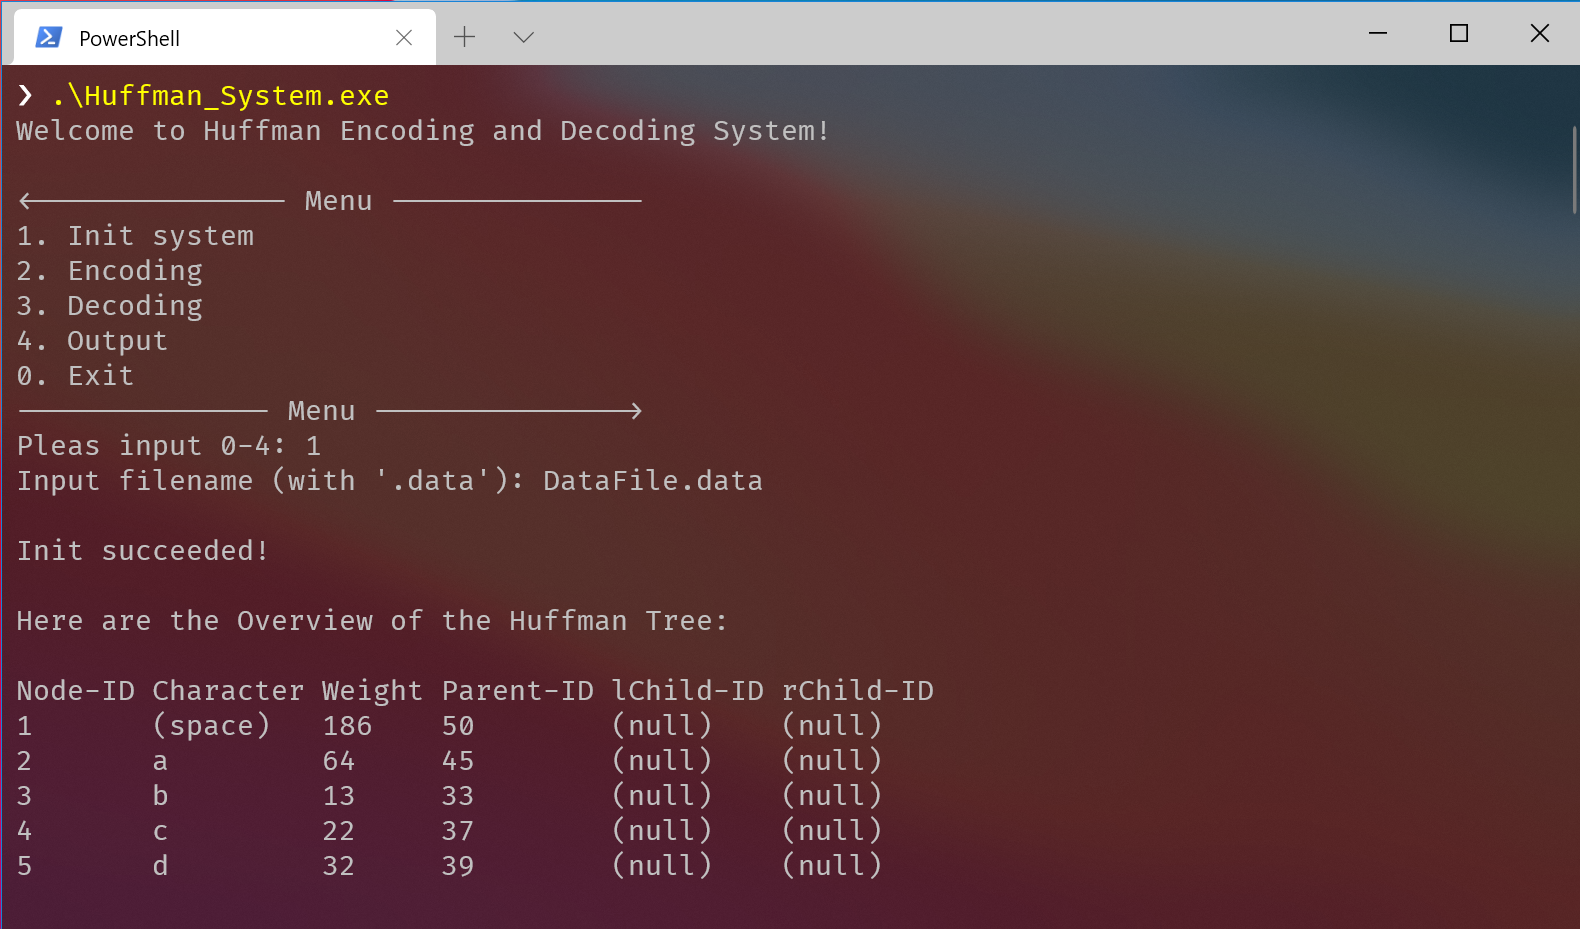
\includegraphics[width=0.8\textwidth]{测试1.png}

        \vspace{1em}
        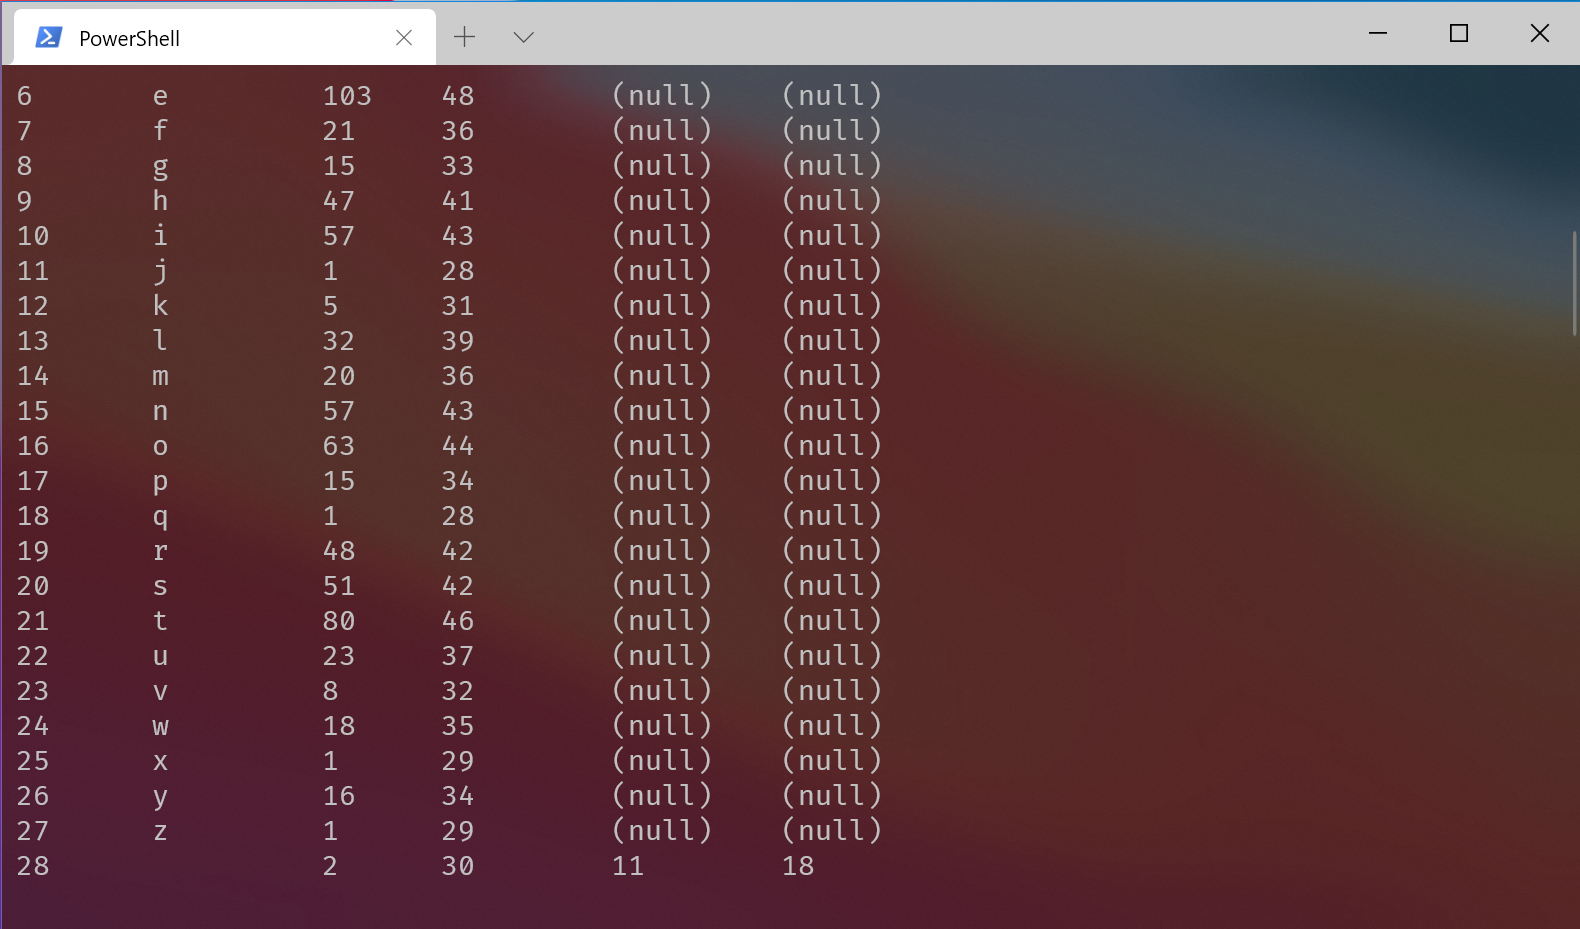
\includegraphics[width=0.8\textwidth]{测试2.png}

        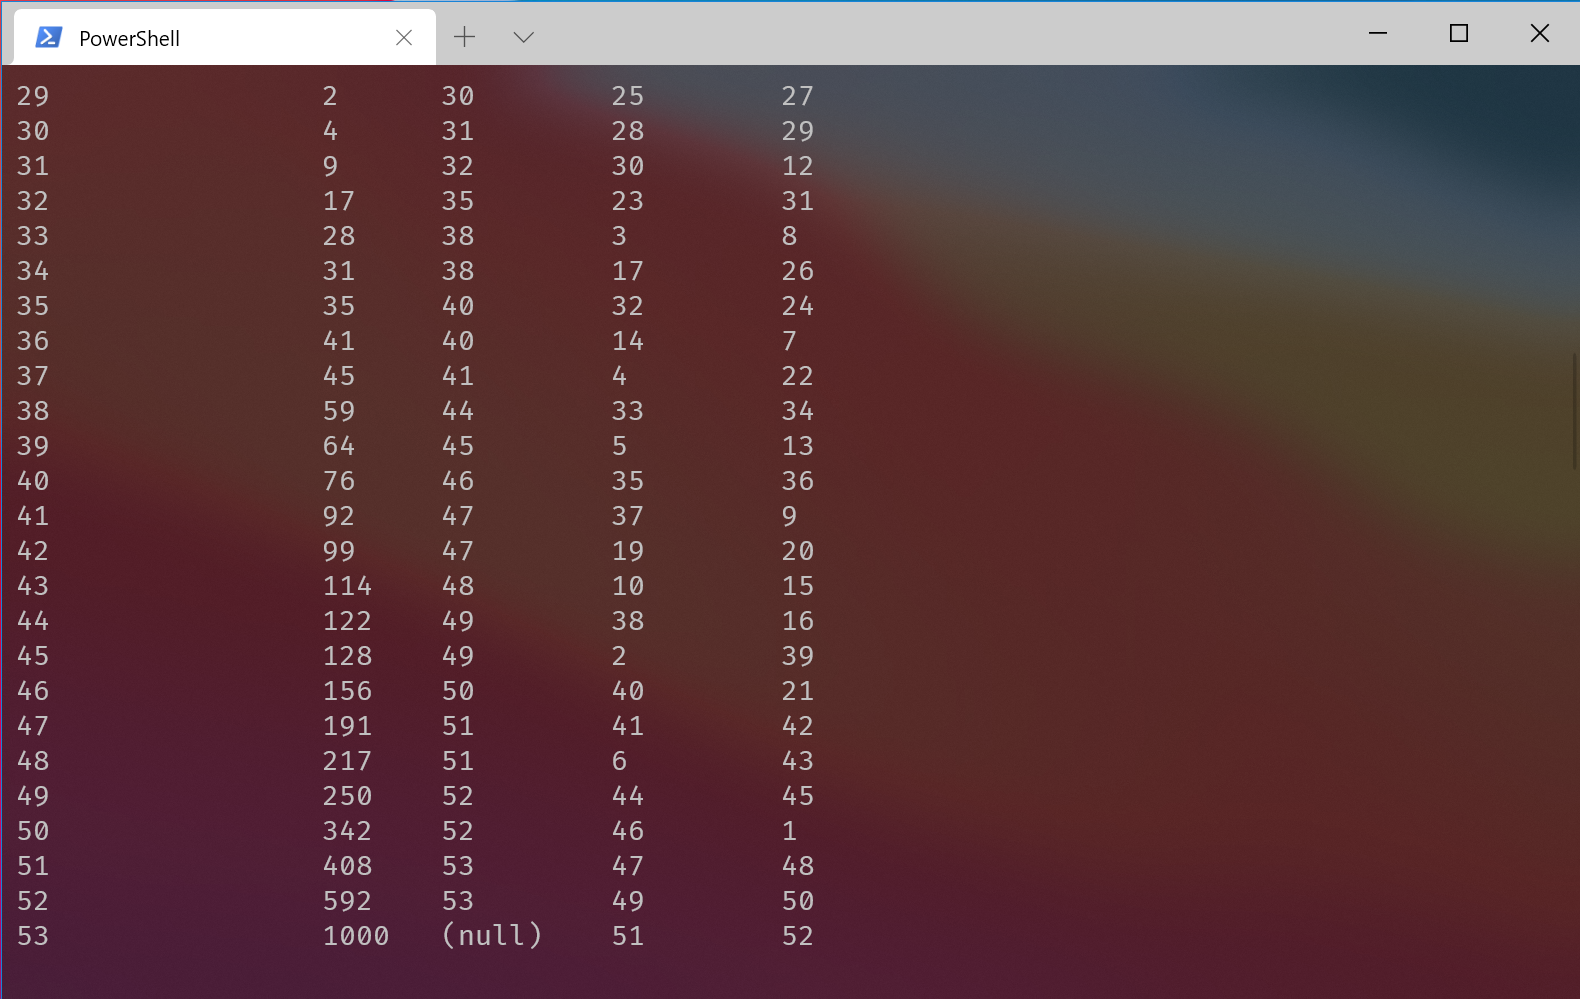
\includegraphics[width=0.8\textwidth]{测试3.png}
    \end{center}

    \subsection{编码字符串}
    对ToBeTran.data中的字符串进行编码,并将结果写入Code.txt中。
    \begin{center}
        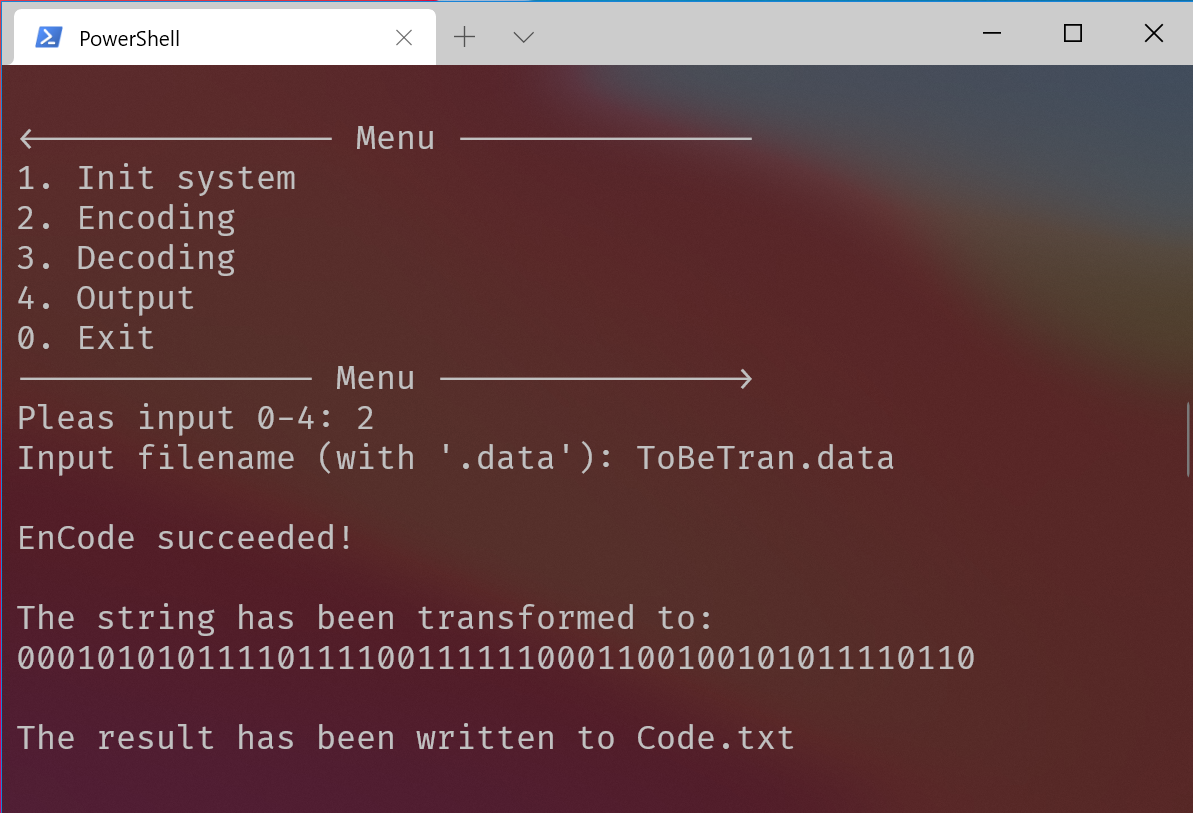
\includegraphics[width=0.8\textwidth]{测试4.png}
    \end{center}

    \subsection{译码二进制哈夫曼编码}
    对CodeFile.data中的字符串进行译码,并将结果写入TextFile.txt中。
    \begin{center}
        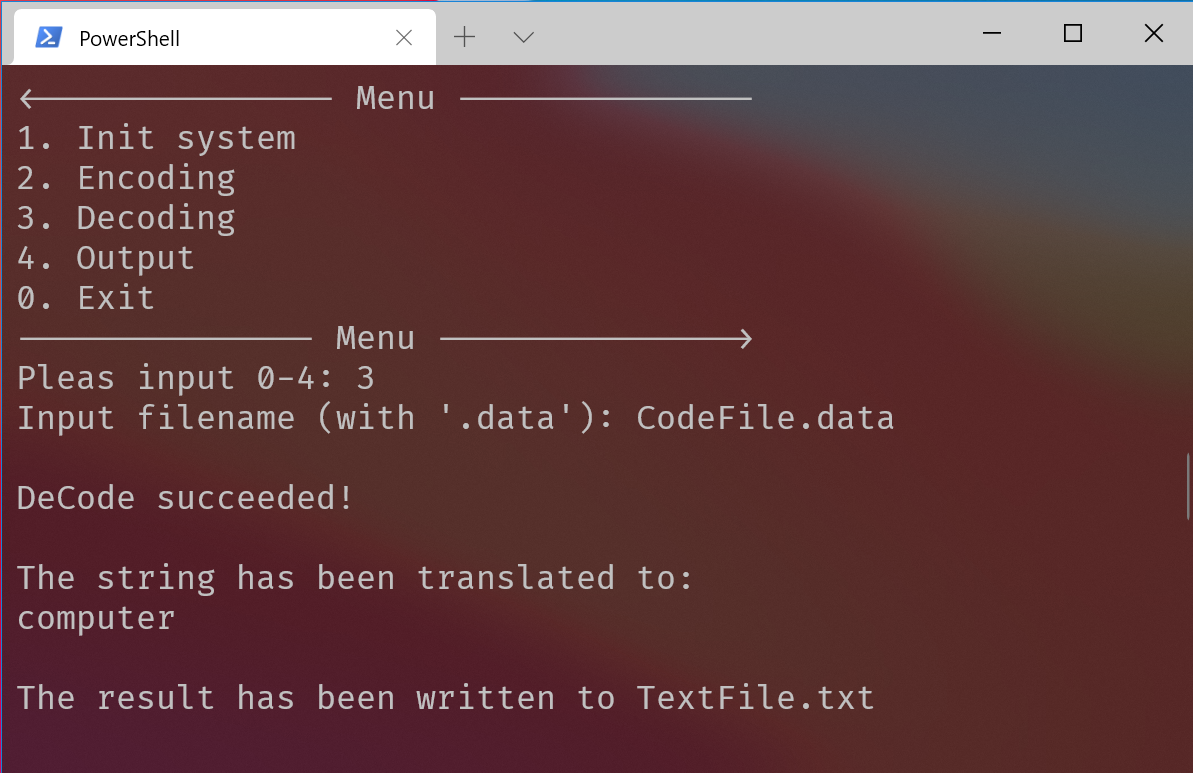
\includegraphics[width=0.65\textwidth]{测试5.png}
    \end{center}

    \subsection{输出}
    展示DataFile.data中出现的字符及其频率;
    输出ToBeTran.data及其报文Code.txt;
    输出CodeFile.data及其原文TextFile.txt。

    \begin{center}
        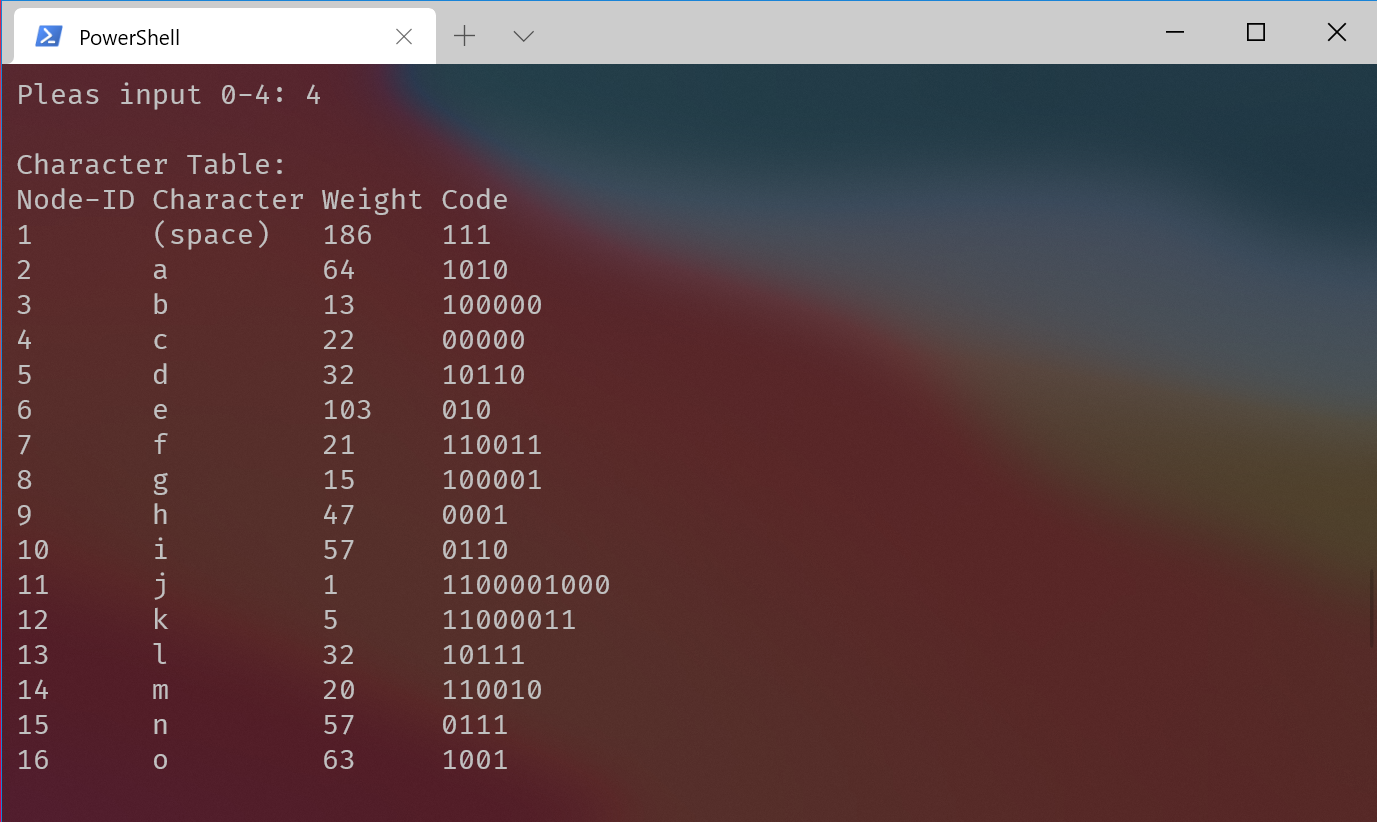
\includegraphics[width=0.65\textwidth]{测试6.png}
        
        \vspace{1em}
        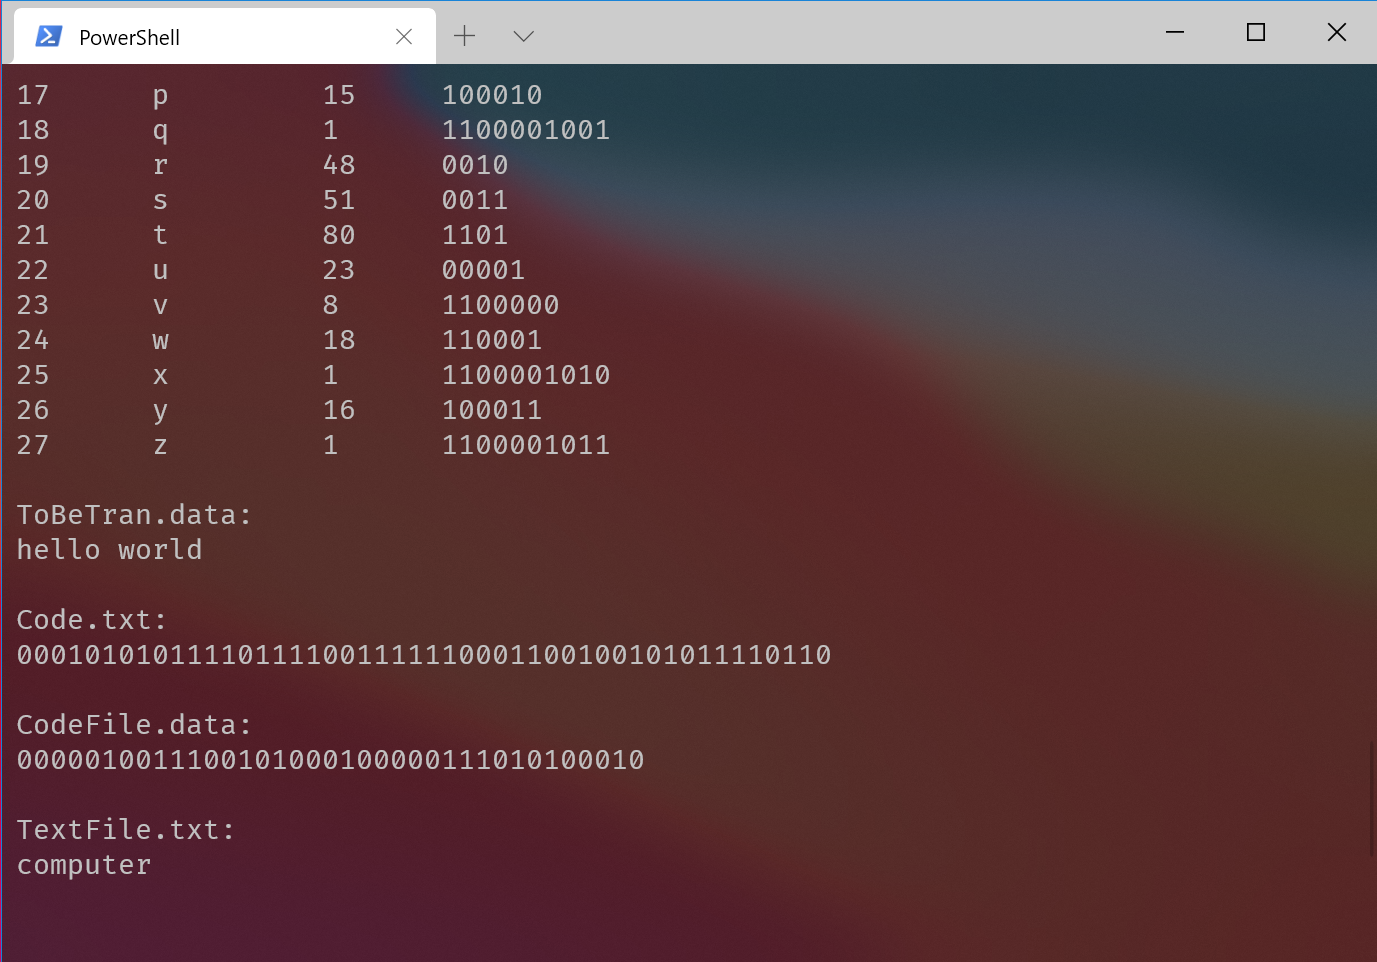
\includegraphics[width=0.65\textwidth]{测试7.png}
    \end{center}
    \section{总结}
    通过本次项目实践,理解了哈夫曼树的特征及应用,掌握了哈夫曼树的构造算法设计。
    熟悉了字符的哈夫曼编码和译码,并能够通过哈夫曼树进行编码和译码操作。通过哈夫曼程序
    的编写,对计算机处理编码问题有了感性的理解,并将树、哈夫曼等知识得到实际应用。
    \section{附录}
    本项目实例使用CMake构建,并要求编译器为 G++ ,使用的操作系统是 Windows。
    
    项目主要文件清单:
    
    \dirtree{%
        .1 /\DTcomment{项目根目录}.
        .2 bin\DTcomment{输出文件夹}.
        .3 CodeFile.data\DTcomment{用以译码的示例文件}.
        .3 DataFile.data\DTcomment{用以构造哈夫曼树的示例文件}.
        .3 Huffman\_System.exe\DTcomment{已经编译的可执行文件}.
        .3 ToBeTran.data\DTcomment{用以编码的示例文件}.
        .2 CMakeLists.txt\DTcomment{CMake 项目配置文件}.
        .2 docs\DTcomment{项目文档目录}.
        .3 images\DTcomment{文档使用的图片资源}.
        .3 project3.pdf\DTcomment{项目文档}.
        .3 project3.tex\DTcomment{项目文档\LaTeX 源文件}.
        .2 src\DTcomment{源代码}.
        .3 main.cpp\DTcomment{主程序}.
        .3 Maze.h\DTcomment{Huffman类头文件}.
    }

    这些源文件可以在 \url{https://github.com/DianDengJun/Course-Design/tree/main/Winter/Project3} 中查看。
    
    构建本实例的命令(Bash 或 Powershell)如下:
    
    进入根目录,执行:
    
    \begin{verbatim}
        mkdir build
        cd build
        cmake -G "MinGW Makefiles" ..
        make # 或者是 mingw32-make
    \end{verbatim}

    然后进入bin目录运行Huffman\_System.exe。

    \begin{verbatim}
        cd ../bin
        ./Huffman_System
    \end{verbatim}
\end{document}